\subsection{Calibración del sistema de visión}
\label{calibracion}
Para una correcta percepción del entorno es necesario realizar una calibración de la cámara para corregir las distorsiones producidas en la imagen por la lente y el sensor de la misma. La cámara posee dos tipos de distorsión: la radial, generada por la lente y que produce la curvatura de las líneas rectas de la imagen, y la tangencial, producida por un desalineamiento de la lente con el plano del sensor, de forma que ambos no se encuentran paralelos. La distorsión tangencial provoca que ciertas zonas de la imagen parezcan más cercanas de lo que realmente están.\\

Las fórmulas que modelan la distorsión radial son las siguientes:
\[x_{corrected} = x (1 + k_1 r^2 + k_2 r^4 + k_3 r^6)\]
\[y_{corrected} = y (1 + k_1 r^2 + k_2 r^4 + k_3 r^6)\]
~\\
 
La distorsión tangencial se modela con las siguientes fórmulas:
\[x_{corrected} = x + \left[2 p_1 x y + p_2 (r^2 + 2 x^2) \right] \]
\[y_{corrected} = y + \left[p_1 (r2 + 2 y^2) + 2 p_2 x y \right] \]
~\\

En total, la distorsión la modelaremos con 5 parámetros: $(k_1 ~ k_2 ~ p_1 ~ p_2 ~ k_3)$\\

También es necesario obtener los parámetros intrínsecos, que son propios de la cámara, como la distancia focal y el centro óptico, así como los parámetros extrínsicos de la cámara,posición y orientación respecto de un sistema de coordenadas 3D.\\

La matriz de la cámara expresa estos parámteros intrínsecos en una sola matriz:
\[camera ~matrix = \begin{bmatrix} f_x & 0 & c_x \\ 0 & f_y & c_y \\ 0 & 0 & 1 \end{bmatrix}\]
Donde $(f_x, f_y)$ son las distancias focales en los ejes x e y, y  las coordenadas del centro óptico son $(c_x, c_y)$.\\

Para realizar la calibración de la cámara es necesario un patrón de calibración como el de la figura \ref{fig:patron_calibracion}, de dimensiones conocidas. Las bibliotecas OpenCV poseen funciones capaces de reconocer y detectar automáticamente los vértices de los cuadrados y, conociendo su posición dentro del patrón y las dimensiones del mismo en la realidad, calcular los parámetros de la cámara.\\

\begin{figure}[H]
        \centering
        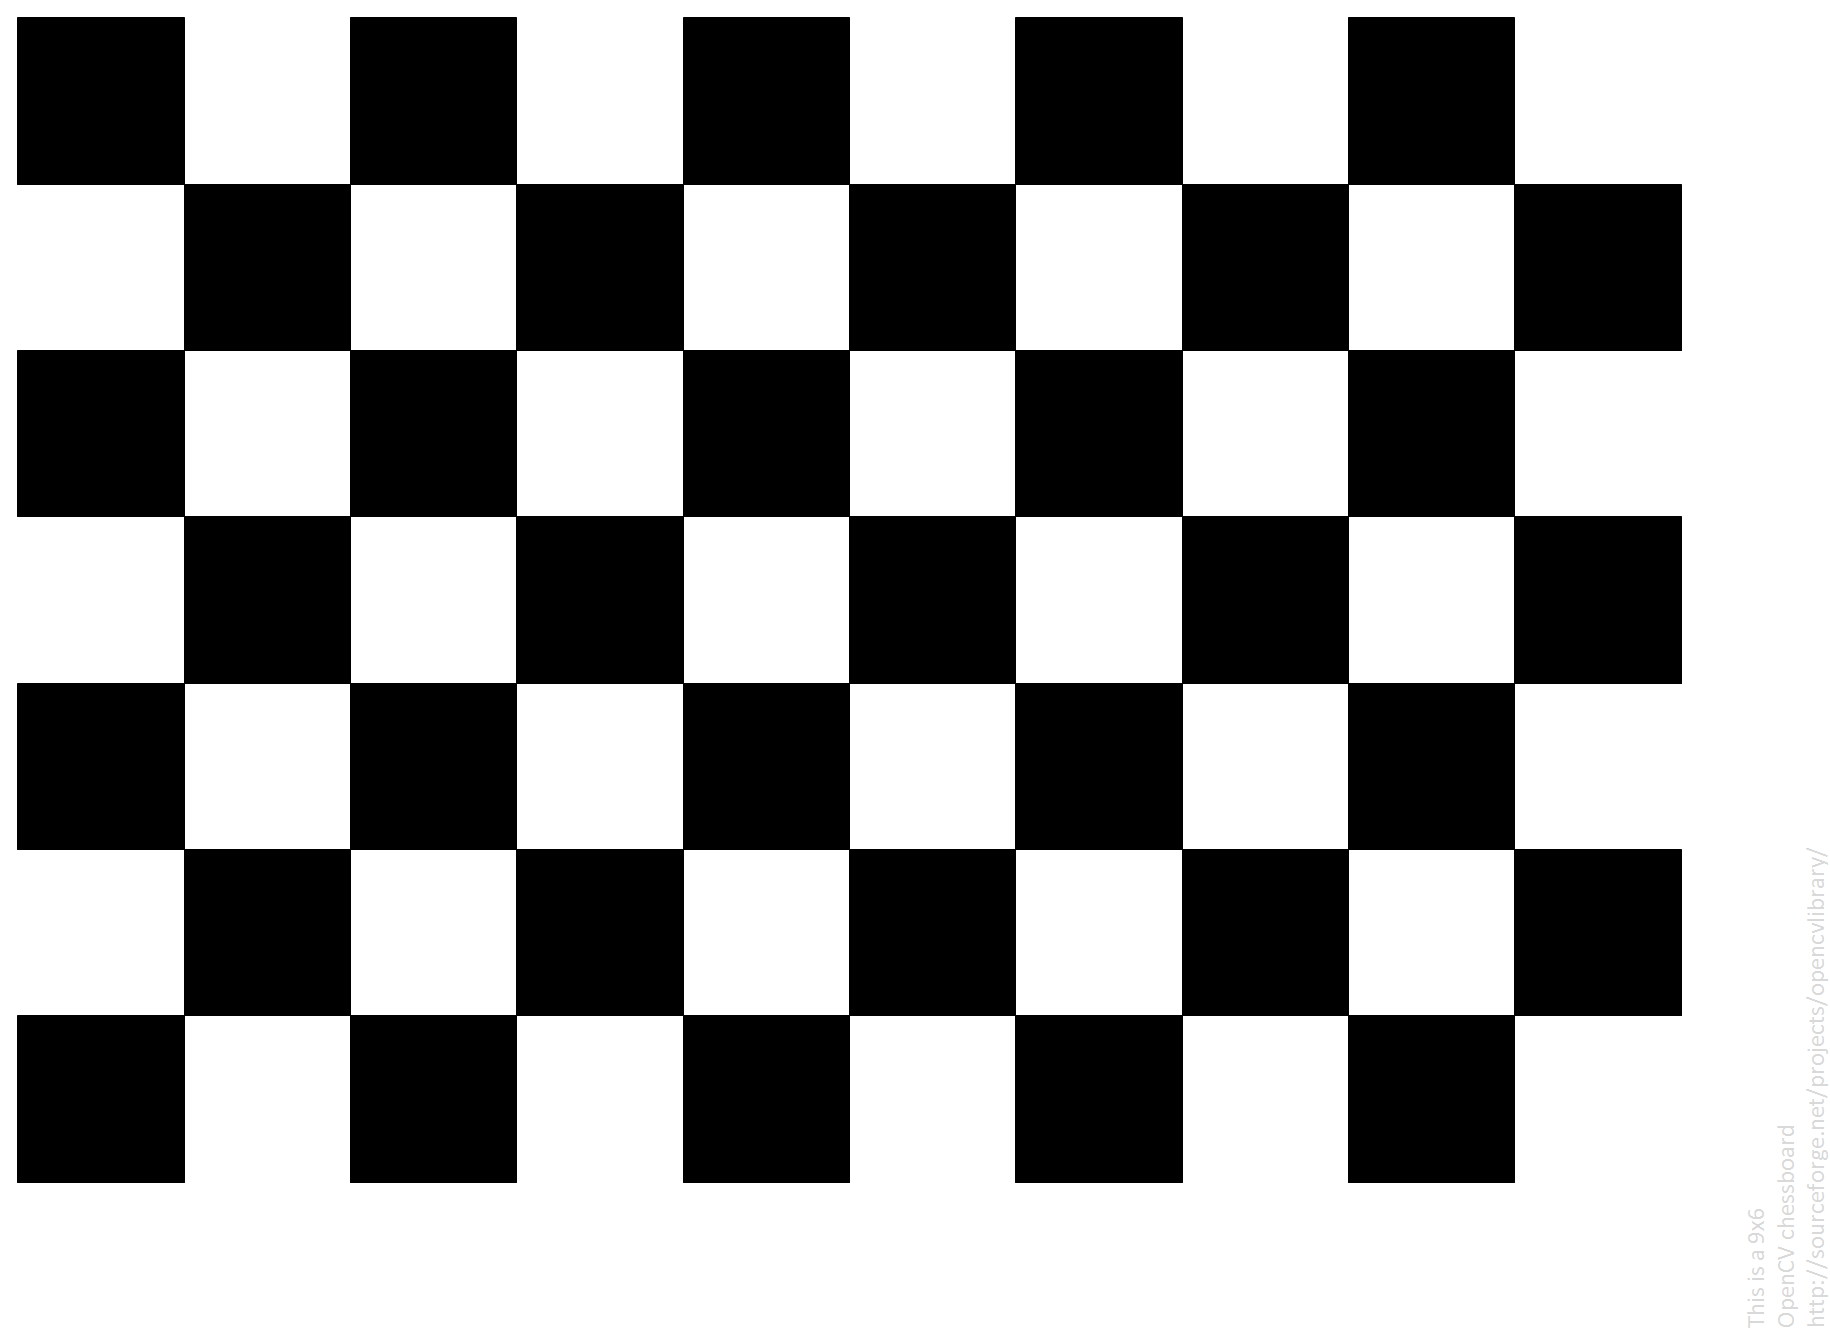
\includegraphics[width=0.5\textwidth]{images/pattern.png}
        \caption{Patrón de calibración proporcionado por OpenCV}
        \label{fig:patron_calibracion}
\end{figure} 

El proceso es el siguiente. En primer lugar se coloca la cámara fija y se realizan una serie de fotos del patrón de calibración en distintas posiciones y orientaciones. Se extraen de estas imágenes los puntos correspondientes a los vértices de los cuadrados del patrón (figura \ref{fig:deteccion_patron}), que OpenCV usa para calcular tanto los parámetros de la distorsión como los parámetros intrínsecos de la cámara.\\

\begin{figure}[H]
        \centering
        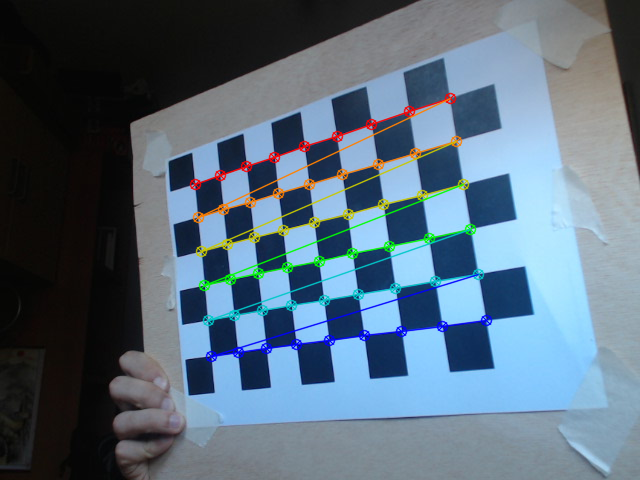
\includegraphics[width=0.5\textwidth]{images/calibration_pattern_detected.png}
        \caption{OpenCV detectando el patrón de calibración}
        \label{fig:deteccion_patron}
\end{figure} 

Una vez obtenidos estos parámetros, se almacenan en un archivo de forma que puedan ser cargados posteriormente. Usando estos archivos, es posible rectificar la imagen para eliminar la distorsión usando la función undistort de OpenCV, y posteriormente se recorta la región de interés de la imagen.\\



\subsection{Procesamiento del entorno}
\label{procesamiento}

El primer paso del algoritmo de planificación y control es la extracción de información del entorno a través de visión artificial. Al no poseer ningún tipo de sensor, toda la información que posee el controlador del robot se obtiene a través del sistema de visión.\\

\begin{figure}[H]
        \centering
        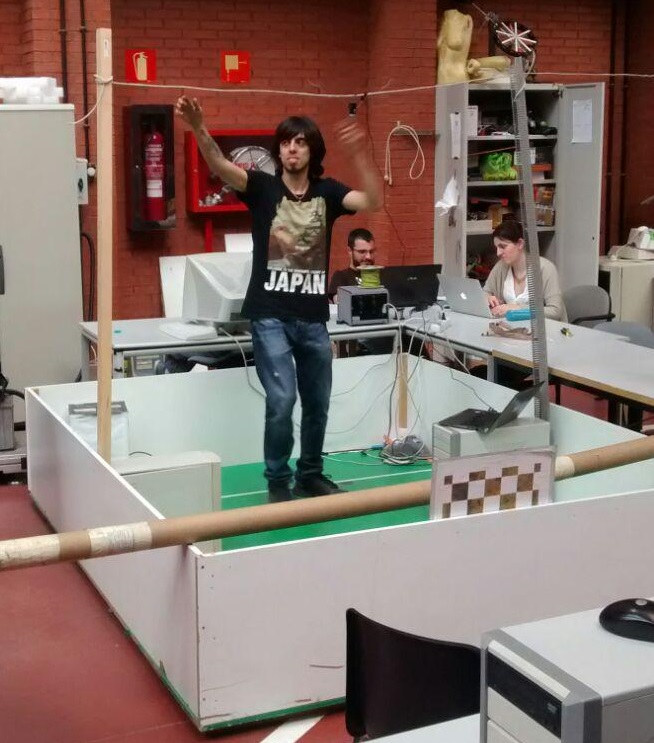
\includegraphics[width=0.4\textwidth]{images/escenario.jpg}
        \caption{David colocando la estructura de soporte de la cámara cenital}
        \label{fig:foto_estructura_nave}
\end{figure} 

El entorno es captado a través de una cámara cenital, fijada a una estructura de soporte (figura \ref{fig:foto_estructura_nave}). El suelo del entorno, un escenario del concurso CEABOT, está pintado de un llamativo tono de verde. Para su localización, el robot lleva en su parte superior un marcador fiduciario formado por un rectángulo de dos colores, negro y azul (figura \ref{fig:marcador_fiduciario}). Al poseer dos colores es posible extraer tanto la posición como la orientación del robot a través de la cámara.\\

\begin{figure}[H]
        \centering
        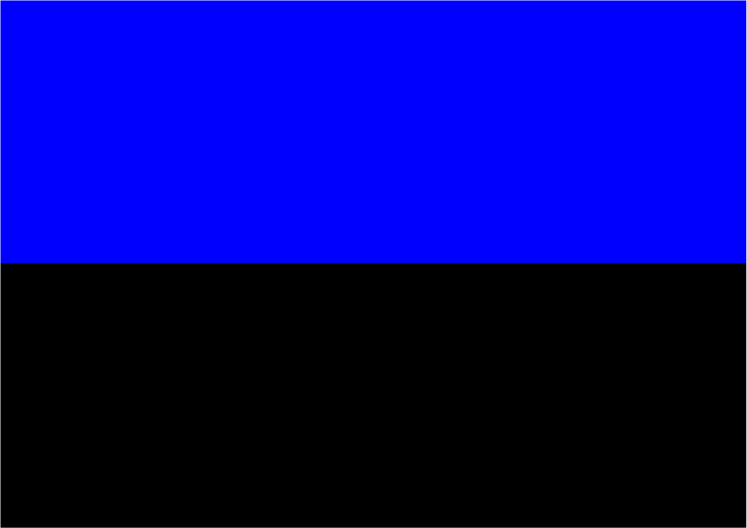
\includegraphics[width=0.4\textwidth]{images/marcador.png}
        \caption{Marcador fiduciario usado para el tracking del robot}
        \label{fig:foto_estructura_nave}
\end{figure} 

Para la detección de obstáculos se utiliza una segmentación del color verde, aplicando una umbralización en el espacio de color HSV. La máscara resultante se procesa con una apertura usando un kernel rectangular de 5x5 píxeles, para reducir el ruido, y se lleva a cabo un etiquetado de objetos sobre la imagen binaria filtrada. Estos contornos, posteriormente, son también filtrados por tamaño y área, y simplificados.\\

A partir de los contornos de estos obstáculos se genera una imagen binaria que es utilizada como mapa para el algoritmo de planificación (figura \ref{fig:map}).\\

\begin{figure}[H]
        \centering
        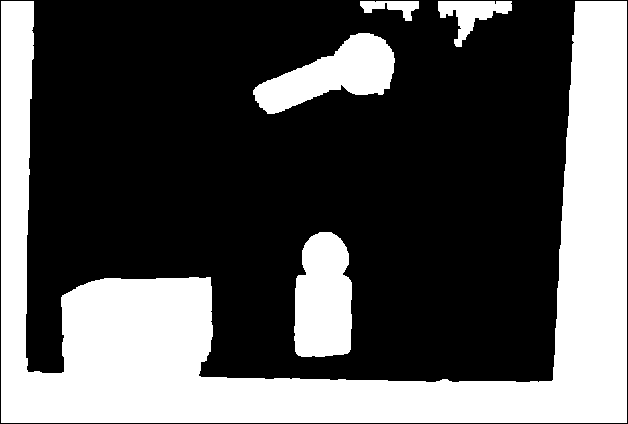
\includegraphics[width=0.4\textwidth]{images/map.png}
        \caption{Mapa del entorno obtenido a partir de los contornos de los obstáculos segmentados.}
        \label{fig:foto_estructura_nave}
\end{figure} 

El marcador del robot se extrae mediante una segmentación del color azul, llevada a cabo también umbralizando en el espacio HSV y realizando el mismo filtrado que en el caso del color verde. Para una detección robusta del color negro del marcador, y para evitar reflejos producidos por una iluminación no controlada, el marcador completo se detecta buscando entre los obstáculos detectados el que posea un rectángulo azul en su interior, que es identificado y etiquetado como robot.\\ 

La posición del robot se obtiene calculando el centro del contorno del robot, y la orientación usando el vector que conecta el centro de dicho contorno con el centro del contorno azul, midiendo su orientación con respecto al eje X.\\

Por último, para la detección de la lata, se comprueban todos los obstáculos buscando aquellos que tengan forma circular. Esta forma circular se calcula teniendo en cuenta la proporción entre el área del contorno y el área del menor circulo que incluye el contorno, que es aproximadamente 1 en el caso de que el contorno sea totalmente circular. Para que la segmentación no etiquete obstáculos circulares como latas, se realiza también un filtrado de candidatos por tamaño, reduciendo así el número de posibles falsos positivos.\\

La figura \ref{fig:segmentation} muestra el resultado de la segmentación. Los contornos amarillos indican los obstáculos, los círculos azules son las latas (objetivos) detectadas y el rectángulo magenta rodea al robot, cuya orientación queda indicada con una línea cyan.\\

\begin{figure}[H]
        \centering
        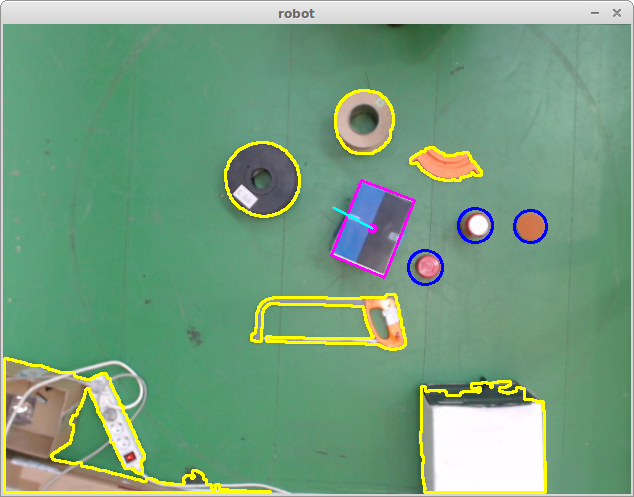
\includegraphics[width=0.4\textwidth]{images/segmentation.png}
        \caption{Resultado de la segmentación}
        \label{fig:segmentation}
\end{figure} 